%!TEX root = ../BUSystematics.tex

\graphicspath{{Body/Figures/Pileup/}{Body/Figures/Pileup/Amplitude/}{Body/Figures/Pileup/TimeShift/}}

\section{Pileup Systematic Errors}

\subsection{Amplitude}

The pileup amplitude error is evaluated by applying a multiplier to the amplitude of the pileup correction and refitting. Multipliers were applied in steps of 0.01 from 0.9 to 1.1, and the resulting R vs pileup multiplier plot is fit to determine the sensitivity of R to the pileup multiplier. The uncertainty in the multiplier is determined as the width of the parabola in the \chisq vs the pileup multiplier. The systematic error on \R is then calculated as 
    \begin{align}
        \delta R = \sigma_{P_{m}} \times \frac{dR}{dP_{m}},
    \end{align}
where $P_{m}$ is the value of the pileup multiplier. \figref{fig:PMscan} shows the scan results for the 9d dataset. \tabref{tab:systematicError_pileupMultplier} gives the systematic errors for the Run~1 datasets.


\begin{figure}
\centering
    \begin{subfigure}[t]{0.45\textwidth}
        \centering
        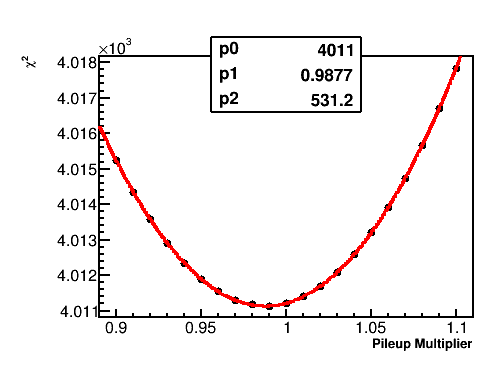
\includegraphics[width=\textwidth]{TMethod_Chi2_Vs_PileupMultiplier_Canv}
        \caption{T-Method \chisq versus pileup multiplier. The parabolic fit equation used was $y = p_{2}(x - p_{1})^{2} + p_{0}.$}
    \end{subfigure}% %you need this % here to add spacing between subfigures
    \hspace{1cm}
    \begin{subfigure}[t]{0.45\textwidth}
        \centering
        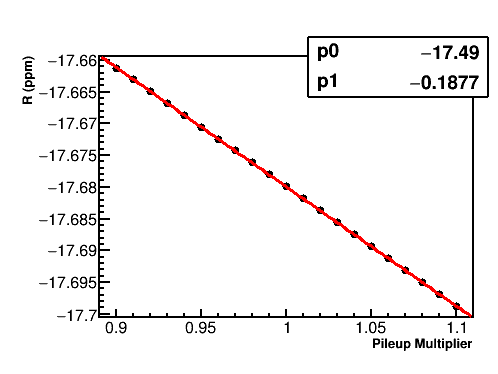
\includegraphics[width=\textwidth]{TMethod_R_Vs_PileupMultiplier_Canv}
        \caption{T-Method $R$ versus pileup multiplier. The parameter $p_{1}$ gives the sensitivity of $R$ to the value of the pileup multiplier, with units in ppm.}
    \end{subfigure}

    \begin{subfigure}[t]{0.45\textwidth}
        \centering
        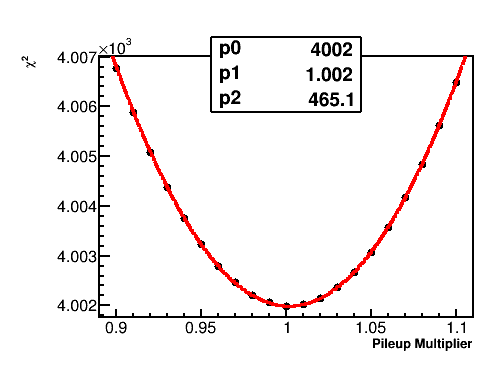
\includegraphics[width=\textwidth]{FullRatio_Chi2_Vs_PileupMultiplier_Canv}
        \caption{R-Method \chisq versus pileup multiplier. The parabolic fit equation used was $y = p_{2}(x - p_{1})^{2} + p_{0}.$}
    \end{subfigure}% %you need this % here to add spacing between subfigures
    \hspace{1cm}
    \begin{subfigure}[t]{0.45\textwidth}
        \centering
        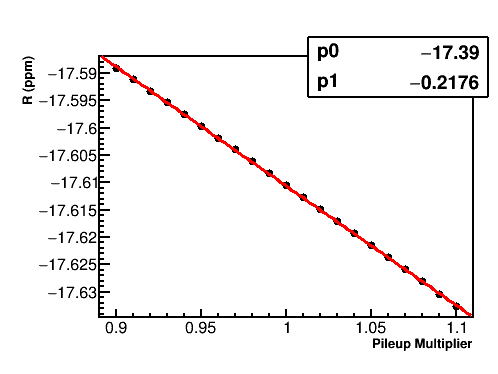
\includegraphics[width=\textwidth]{FullRatio_R_Vs_PileupMultiplier_Canv}
        \caption{R-Method $R$ versus pileup multiplier. The parameter $p_{1}$ gives the sensitivity of $R$ to the value of the pileup multiplier, with units in ppm.}
    \end{subfigure}
\caption[Pileup multiplier scan]{Pileup multiplier scan. Data are from the 9d dataset.}
\label{fig:PMscan}
\end{figure}



\begin{table}
\centering
\renewcommand{\arraystretch}{1.2}
\begin{tabularx}{0.65\linewidth}{XYY}
  \hline
    \multicolumn{3}{c}{\textbf{Systematic Error due to Pileup Amplitude}} \\
  \hline\hline
    Dataset & \thead{T-Method} & \thead{R-Method} \\
  \hline
    60h & 21.7 & 19.9 \\
    HighKick & 11.4 & 11.4 \\
    9d & 8.1 & 10.1 \\ 
    Endgame & 10.1 & 9.4 \\
  \hline
\end{tabularx}
\caption[Systematic error due to pileup amplitude]{Systematic error due to the pileup amplitude. Units are in ppb.}
\label{tab:systematicError_pileupMultplier}
\end{table}





\subsection{Cluster Time Model}

The time of a constructed doublet in the pileup construction is set as the energy weighted time of the two singlets plus half the gap time. Previously the error was calculated by scanning over an additional time shift and then applying a conservative uncertainty of \ns{2.5}. The results of such a scan can be seen in \figref{fig:PTSscan}. If this procedure is used then the systematic error on \R is less than 15 ppb for all datasets.

That is however a pretty conservative approach. If I instead use the most energetic singlet time as the doublet time, then the $\Delta R$ is less than \ppb{1} for all datasets. If I instead set the doublet time as either the first singlet time, or the second singlet time, then the $\Delta R$'s are given in \tabref{tab:systematicError_clusterTimeDeltas} and range around 5-6~ppb. I take as my systematic error half this range for all datasets. The final systematic errors are given in \tabref{tab:systematicError_clusterTimeModel}.



\begin{figure}
\centering
    \begin{subfigure}[t]{0.45\textwidth}
        \centering
        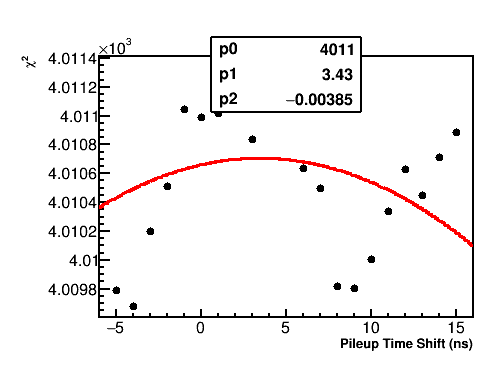
\includegraphics[width=\textwidth]{TMethod_Chi2_Vs_PileupTimeShift_Canv}
        \caption{T-Method \chisq versus pileup time shift. There is no clear minimum.}
    \end{subfigure}% %you need this % here to add spacing between subfigures
    \hspace{1cm}
    \begin{subfigure}[t]{0.45\textwidth}
        \centering
        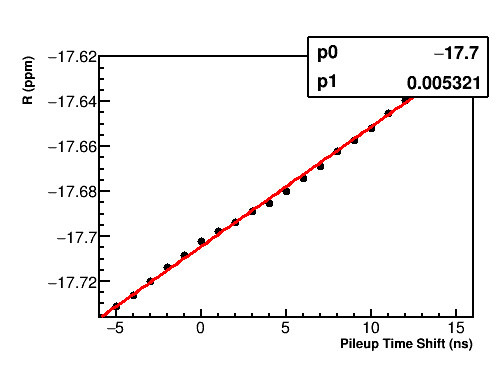
\includegraphics[width=\textwidth]{TMethod_R_Vs_PileupTimeShift_Canv}
        \caption{T-Method $R$ versus pileup time shift. The parameter $p_{1}$ gives the sensitivity of $R$ to the value of the pileup time shift, with units in ppm.}
    \end{subfigure}
\caption[Pileup time shift scan]{Pileup time shift scan for the T-Method. The R-Method plots look the same. Data are from the 9d dataset.}
\label{fig:PTSscan}
\end{figure}


\begin{table}
\centering
\renewcommand{\arraystretch}{1.2}
\begin{tabularx}{0.85\linewidth}{@{\extracolsep{\fill}}XYY|YY}
  \hline
    \multicolumn{5}{c}{$\Delta R$ with first and last singlet times} \\
  \hline\hline
            & \multicolumn{2}{c|}{T-Method} & \multicolumn{2}{c}{R-Method } \\
    Dataset & \thead{First Time} & \multicolumn{1}{c|}{Last Time} & \thead{First Time} & \thead{Last Time}  \\
  \hline
    60h & -5.5 & 4.6 & -8.0 & 4.8 \\
    HighKick & -5.0 & 4.3 & -5.6 & 4.0 \\
    9d & -5.4 & 5.6 & -5.8 & 5.4 \\ 
    Endgame & -4.5 & 4.4 & -5.2 & 4.3 \\
  \hline
\end{tabularx}
\caption[]{$\Delta R$ when applying the two singlet times as the doublet times. Units are in ppb.}
\label{tab:systematicError_clusterTimeDeltas}
\end{table}



\begin{table}
\centering
\renewcommand{\arraystretch}{1.2}
\begin{tabularx}{0.65\linewidth}{@{\extracolsep{\fill}}XYY}
  \hline
    \multicolumn{3}{c}{\textbf{Systematic Error due to Cluster Time Model}} \\
  \hline\hline
    Dataset & \thead{T-Method} & \thead{R-Method} \\
  \hline
    60h & 5.1 & 6.4 \\
    HighKick & 4.6 & 4.8 \\
    9d & 5.5 & 5.6 \\ 
    Endgame & 5.0 & 4.8 \\
  \hline
\end{tabularx}
\caption[Systematic error due to cluster time model]{Systematic error due to cluster time model. Units are in ppb.}
\label{tab:systematicError_clusterTimeModel}
\end{table}











\subsection{Cluster Energy Model}

\begin{table}
\centering
\renewcommand{\arraystretch}{1.2}
\begin{tabularx}{0.65\linewidth}{@{\extracolsep{\fill}}XYY}
  \hline
    \multicolumn{3}{c}{\textbf{Systematic Error due to Cluster Energy Model}} \\
  \hline\hline
    Dataset & \thead{T-Method} & \thead{R-Method} \\
  \hline
    60h & 0.0 & 0.0 \\
    HighKick & 0.0 & 0.0 \\
    9d & 0.0 & 0.0 \\ 
    Endgame & 0.0 & 0.0 \\
  \hline
\end{tabularx}
\caption[Systematic error due to cluster energy model]{Systematic error due to cluster energy model. Units are in ppb.}
\label{tab:systematicError_clusterEnergyModel}
\end{table}

\subsection{Rate Error}

\begin{table}
\centering
\renewcommand{\arraystretch}{1.2}
\begin{tabularx}{0.65\linewidth}{@{\extracolsep{\fill}}XYY}
  \hline
    \multicolumn{3}{c}{\textbf{Systematic Error due to Pileup Rate Error}} \\
  \hline\hline
    Dataset & \thead{T-Method} & \thead{R-Method} \\
  \hline
    60h & 0.0 & 0.0 \\
    HighKick & 0.0 & 0.0 \\
    9d & 0.0 & 0.0 \\ 
    Endgame & 0.0 & 0.0 \\
  \hline
\end{tabularx}
\caption[Systematic error due to pileup rate error]{Systematic error due to pileup rate error. Units are in ppb.}
\label{tab:systematicError_pileupRateError}
\end{table}

\subsection{Unseen Pileup}

\begin{table}
\centering
\renewcommand{\arraystretch}{1.2}
\begin{tabularx}{0.65\linewidth}{@{\extracolsep{\fill}}XYY}
  \hline
    \multicolumn{3}{c}{\textbf{Systematic Error due to Unseen Pileup}} \\
  \hline\hline
    Dataset & \thead{T-Method} & \thead{R-Method} \\
  \hline
    60h & 0.0 & 0.0 \\
    HighKick & 0.0 & 0.0 \\
    9d & 0.0 & 0.0 \\ 
    Endgame & 0.0 & 0.0 \\
  \hline
\end{tabularx}
\caption[Systematic error due to unseen pileup]{Systematic error due to unseen pileup. Units are in ppb.}
\label{tab:systematicError_unseenPileup}
\end{table}

\subsection{Triple Pileup Correction}

\begin{table}
\centering
\renewcommand{\arraystretch}{1.2}
\begin{tabularx}{0.65\linewidth}{@{\extracolsep{\fill}}XYY}
  \hline
    \multicolumn{3}{c}{\textbf{Systematic Error due to Triple Pileup Correction}} \\
  \hline\hline
    Dataset & \thead{T-Method} & \thead{R-Method} \\
  \hline
    60h & 0.0 & 0.0 \\
    HighKick & 0.0 & 0.0 \\
    9d & 0.0 & 0.0 \\ 
    Endgame & 0.0 & 0.0 \\
  \hline
\end{tabularx}
\caption[Systematic error due to triple pileup correction]{Systematic error due to triple pileup correction. Units are in ppb.}
\label{tab:systematicError_triplePileupCorrection}
\end{table}





% \begin{table}
% \centering
% \renewcommand{\arraystretch}{1.2}
% \begin{tabularx}{0.65\linewidth}{@{\extracolsep{\fill}}XYY}
%   \hline
%     \multicolumn{3}{c}{\textbf{Systematic Error due to}} \\
%   \hline\hline
%     Dataset & \thead{T-Method} & \thead{R-Method} \\
%   \hline
%     60h & 0.0 & 0.0 \\
%     HighKick & 0.0 & 0.0 \\
%     9d & 0.0 & 0.0 \\ 
%     Endgame & 0.0 & 0.0 \\
%   \hline
% \end{tabularx}
% \caption[Systematic error due to]{Systematic error due to. Units are in ppb.}
% \label{tab:systematicError_}
% \end{table}






